\section{Motivation}
\label{s:motivation}

% - what is concurrency bugs
% - characteristics of concurrency bugs
% - challenges / design requirements
% - limitations of existing approaches

In this section, we first describe how concurrency bugs manifest
depending on thread interleaving.
%
We then define design requirements to effectively discover concurrency
bugs in the kernel and summarize why existing approaches do not
satisfy the design requirements.


\PP{Manifestation of concurrency bugs}
%
This paper focuses on finding concurrency bugs in system softwares
such as the kernel.
%
A concurrency bug is a bug that manifests depending on the timing of
concurrent events (\eg, memory accesses) that access shared data.
%
More specifically, two instructions \textit{conflict} if \textbf{1)}
they access the same memory location, \textbf{2)} at least one of them
is a store operation, and \textbf{3)} they are executed concurrently.
%
Then, a concurrency bug manifests 


A concurrency bug manifests as \textit{a combined result of
  interleaving of a small number of instructions.}




According to the extensive survey conducted by Shan Lu
\etal~\cite{learningfrommistakes}, most (\ie, more than 90\%)
concurrency bugs manifest depending on the execution order of a small
number (mostly, four) of memory accesses.




% This paper aims to identify data races in system software.
% A data race is behavior in which the output is dependent on
% the sequence or the timing of other non-deterministic events.
% More specifically, a data race occurs when two memory access
% instructions in a target program meet the following three
% conditions: (i) they access the same memory location. (ii)
% at least one is a write instruction. and (iii) they are executed
% concurrently.
% If all above three conditions above are met, the memory
% accesses performed by the two memory instructions can be non-
% deterministic, rendering computational result to vary depending
% on the execution order. Throughout this paper, we use the
% term RacePaircand to denote two memory access instructions
% that may satisfy the three conditions described above (i.e., a
% candidate race pair), and we use RacePairtrue for those that are
% confirmed to meet the three conditions (i.e., a true race pair,
% which is a subset of RacePaircand).
% Data races can be further classified into two groups: benign
% and harmful. A benign race is an expected (or intentional)
% data race by developers, tolerating a potential deviation in the
% computational results. For example, it is common to allow
% data races in maintaining performance counters, as doing so
% can avoid sluggish data contentions on a performance counter
% variable (while tolerating a small error of a counter value). We
% use the term RacePairbenign to refer to two memory instructions
% raising such a benign race.
% A harmful race is a data race that negatively impacts a run-
% time behavior of a program, and we use the term RacePairharm
% for this case. Due to the non-deterministic computational result,
% there can be various aftermaths of a harmful race, including
% deadlocks, raising safety assertions in the kernel, and memory
% safety violations (including stack/heap buffer overflows, use-
% after-free, and double-free), etc. We note that these aftermaths
% are critical to kernel’s reliability and security: deadlocks may
% make the kernel unresponsive, violating safety assertions may
% cause a reboot the kernel, and memory safety violations allow
% a privilege escalation attack. We use the term RacePairharm to
% refer to two memory instructions in this case.
% Summarizing the terminology, RacePaircand refers to two
% memory access instructions that may cause a race, and
% RacePairtrue refers to two instructions that are confirmed to
% cause a race. RacePairtrue can be further classified into two
% groups: RacePairbenign and RacePairharm.


\begin{figure}[t]
  \centering
  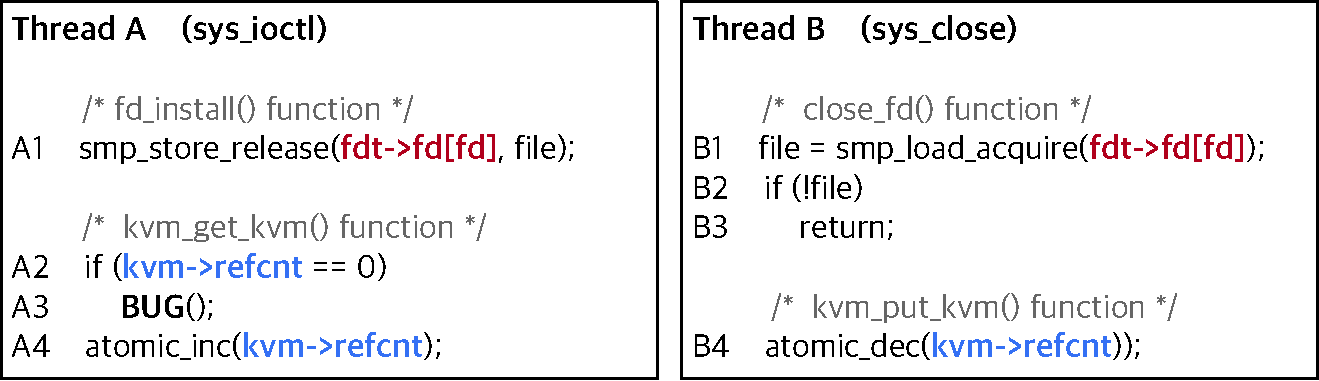
\includegraphics[width=0.95\linewidth]{fig/cve-2017-10661.pdf}
  \caption{Simplified code snippet of CVE-2017-7533. If \texttt{B1} is
    executed between \texttt{A2} and \texttt{A4}, a race condition on
    \texttt{inet->hdrincl} leads to uninitialized stack pointer usage
    on \texttt{rfv}, and an attacker may gain root privileges.}
  \label{fig:cve-2019-6974}
\end{figure}

\dr{I'm rewriting all belows}

% \autoref{fig:cve-2019-6974} describes how an erroneous instance of
% thread interleaving causes a concurrency bug.
% %
% In this example, a NULL-dereference bug may manifest when two system
% calls are executed concurrently: \texttt{mmap()} to map the device
% driver into a user address space and \texttt{ioctl(TRANSACTION)} to
% send an IPC message.


% Assuming \texttt{alloc->vma} and \texttt{alloc->mm} are initially
% \texttt{NULL}, the race condition manifests depending on the execution
% order of four memory accesses, \texttt{A1} and \texttt{A2} in
% thread~A, and \texttt{B1} and \texttt{B4} in thread~B.
% %
% During mapping the device driver into a user address space, thread~A
% sets \texttt{alloc->vma} and \texttt{alloc->mm} to non-NULL pointers
% at \texttt{A1} and \texttt{A2}.
% %
% However, since these store operations are not atomically executed,
% thread~B may intervene in the middle of these two operations.
% %
% In that case, if \texttt{A1} is executed before \texttt{B1}, thread~B
% does not return at \texttt{B3} because thread~B reads a non-NULL
% pointer value through \texttt{alloc->vma}.
% %
% And then if \texttt{B4} is executed before \texttt{A2},
% \texttt{alloc->mm} still remains \texttt{NULL} when thread~B
% increments the reference counter of \texttt{alloc->mm} at \texttt{B4},
% causing a NULL-dereference bug.



% It is noteworthy that the manifestation of a concurrency bug is
% \textit{a combined result of a few conditions on the execution order
%   of instruction pairs that access shared data.}
% %
% In this example, since \texttt{A1} and \texttt{B1} access shared data
% called \texttt{alloc->vma}, the execution order of these two accesses
% may change the kernel's execution. Among the two possible execution
% order of \texttt{A1} and \texttt{B1},
% $\texttt{A1} \rightarrow \texttt{B1}$ is required for the
% NULL-dereference to manifest.
% %
% Similary, the execution order of \texttt{A2} and \texttt{B4} also
% affects the kernel's execution, and
% $\texttt{B4} \rightarrow \texttt{A2}$ is necessary to cause the
% concurrency bug.
% %
% In summary, among all possible conditions on the execution order of
% these instructions, \textit{only}
% $(\texttt{A1} \rightarrow \texttt{B1}) \wedge (\texttt{B4} \rightarrow
% \texttt{A2})$ causes the NULL-dereference bug.


% % In this example, we can confirm that the manifestation of the race
% % condition follows the implications of previous studies; the race
% % condition manifests if \textit{two} scheduling constraints on
% % \textit{four} memory access operations (\ie,
% % $(\texttt{A1} \rightarrow \texttt{B1}) \wedge (\texttt{B4} \rightarrow
% % \texttt{A2})$) are conjunctively satisfied.


% % One of the factors that makes it difficult to find concurrency bugs is
% % that, they may be detected only when a program shows an abnormal
% % behavior.
% % %
% % \autoref{subfig:racecondition} is the example of such concurrency bug.
% % %
% % In this example, the timing of accesses are not correctly
% % contemplated. When instructions are executed in the order of
% % \dr{TODO:}..., the program runs differently than the developer
% % intention, causing a use-after-free bug.
% % %
% % However there are no plain accesses (\ie, all accesses are annotated),
% % and therefore, there is no data race.
% % %
% % By the definition, data race detectors~\cite{tsan, kcsan, krace,
% %   prorace, txrace, crsampler} are not applicable to detect this kind
% % of race conditions.


% % In worse cases, race conditions hardly manifest with the kernel
% % scheduler. In detail, a race condition may manifest only when one
% % thread stalls for a long time while another thread executes numerous
% % instructions.
% % %
% % One could argue that those concurrency bugs are not a threat because
% % it may take too long time, or even impossible to exploit.
% % %
% % However, a recent study, ExpRace~\cite{exprace}, reveals that an
% % attacker can affect the kernel's scheduler using inter-processor
% % interrupts (IPI), and exploit even such concurrency bugs.


% \PP{Design requirements}
% %
% The main goal of this paper is to effectively find out concurrency
% bugs through fuzzing.
% %
% Considering the numerous number of possible instances of thread
% interleaving, we identify two design requirements to explore the
% search space of thread interleaving as follows:

% \begin{itemize}
% \item A fuzzer needs a coverage metric in the concurrency dimension to
%   determine if any interesting interleaving remains
% \item A fuzzer 
% \end{itemize}


% In other words,


% \subsection{Limitation of prior approaches}
% \label{ss:existingapproaches}

% Even though prior approaches achieved their own successes, none of
% them satisfy the two design requirements.

% \PP{}


% \PP{}


% In the perspective of fuzzing, a coverage metric is a paramount gear
% to determine whether a given input is worthy of further mutation.
% %
% If a coverage metric does not represent whether an input has a
% potential to trigger a race condition, a fuzzer may ignore inputs in
% which there are unexplored interleavings, or waste the computing power
% to valueless inputs.
% %
% In this regard, our primary question is whether existing coverage
% metrics in the concurrency dimension are suitable to apprehend
% interleavings potentially causing a race condition, for example,
% $(\texttt{A1} \rightarrow \texttt{B1}) \wedge (\texttt{B4} \rightarrow
% \texttt{A2})$ in \autoref{fig:cve-2019-6974}.



% Unfortunately, we observe that none of existing approaches incorporate
% a proper coverage metric for race conditions.
% %
% A few of existing approaches~\cite{snowboard, razzer} do not adopt a
% coverage in the concurrency dimension at all. Therefore, they do not
% make a decision as to whether a given input is worth further testing.
% %
% Other approaches~\cite{krace, muzz} adopt coverage metrics that are
% not suitable for race conditions as they do not consider a combined
% result of multiple pairs of conflicting accesses. As a consequence,
% race conditions may not be exposed even after the coverages are
% saturated.
% %
% % Consequently, existing approaches have difficulty in distinguishing a
% % given input has a potential to cause an interesting behavior, \ie,
% % a race condition.


% \begin{figure}[t]
%   \centering
%   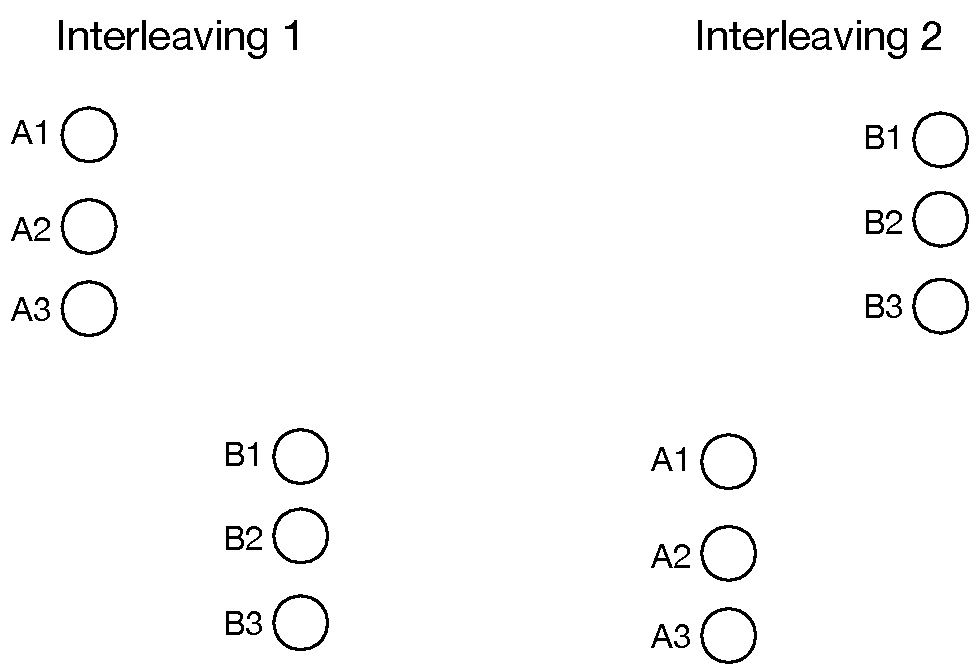
\includegraphics[width=0.98\linewidth]{fig/alias-coverage.pdf}
%   \caption{Three inputs that consist of two concurrent syscalls. For
%     all inputs, thread~A executes the same \texttt{mmap()} syscall
%     while thread~B handles different ioctl requests. For brevity, we
%     describe only conflicting instructions.\dr{Change the name of two
%       ioctls in input 1 and 2}}
%   \label{fig:alias-coverage}
% \end{figure}

% \yj{This is the key paragraph to point out the limitation of previous approaches, but very vague. Make specific claims of why Kraces' alias coverage is insufficient by giving an example.}
% %
% In order to show why comprehending multiple pairs of conflicting
% accesses is important, let us suppose we have three inputs that
% consists of two concurrent syscalls as described in
% \autoref{fig:alias-coverage}.
% %
% For all inputs, thread~A executes a \texttt{mmap()} syscall to map the
% binder driver to a user address space while thread~B handles different
% ioctl requests such that \texttt{ioctl(FREE_BUFFER)},
% \texttt{ioctl(REPLY)}, and \texttt{ioctl(TRANSACTION)} for
% \texttt{Input 1}, \texttt{Input 2}, and \texttt{Input 3} respectively.
% %
% It is worth noting that in \texttt{Input 1} and \texttt{Input 2},
% there is only one pair of conflicting accesses; in \texttt{Input 1},
% the two threads conflict on \texttt{alloc->vma}, and in \texttt{Input
%   2}, the two threads conflict on \texttt{alloc->mm}.



% \begin{figure}[t]
%   \centering
%   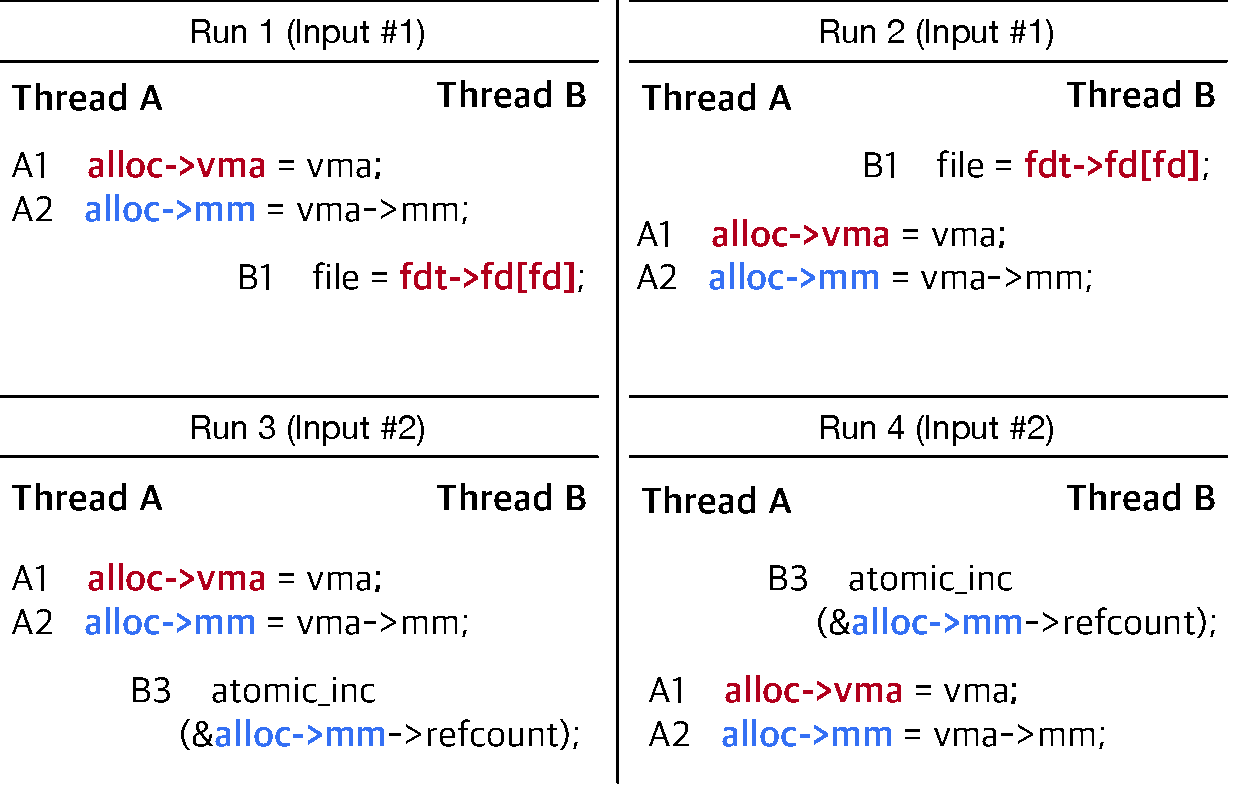
\includegraphics[width=0.9\linewidth]{fig/alias-coverage-interleaving.pdf}
%   \caption{Four interleavings of \texttt{Input 1} and \texttt{Input 2}
%     in \autoref{fig:alias-coverage}. After executing these four
%     interleavings, all possible execution orders of a single
%     conflicting accesses are exhibited.\dr{Run 1 -> Interleaving 1?}}
%   \label{fig:alias-coverage-interleaving}
% \end{figure}

% In this example, if we adopt a coverage metric that focuses on a
% single pair of conflicting accesses (\eg, alias coverage), a fuzzer
% may not recognize that \texttt{Input 3} may exhibit a different
% behavior than \texttt{Input 1} and \texttt{Input 2}~(\ie, a
% NULL-dereference bug).
% %
% \autoref{fig:alias-coverage-interleaving} shows four interleavings
% that exhibits all execution order of a single pair of conflicting
% accesses. If a fuzzer executes \texttt{Input 1} with interleavings in
% \texttt{Run 1} and \texttt{Run 2}, a fuzzer observes execution orders
% such as $\texttt{A1} \rightarrow \texttt{B1}$ (in \texttt{Run 1}) and
% $\texttt{B1} \rightarrow \texttt{A1}$ (in \texttt{Run 2}).
% %
% Similary, if a fuzzer executes \texttt{Input 2} with interleavings in
% \texttt{Run 3} and \texttt{Run 4}, it observes execution orders of
% $\texttt{A2} \rightarrow \texttt{B4}$ (in \texttt{Run 3}) and
% $\texttt{B4} \rightarrow \texttt{A2}$ (in \texttt{Run 4}).
% %
% After executing these four interleavings, \texttt{Input 3} does not
% reveal a new execution order of a single conflicting
% accesses. Therfore, as a Krace state, a fuzzer may de-prioritize
% \texttt{Input 3}, and the race condition may not be found.

% In summary, in order to determine whether an input shows interesting
% behaviors or not, a fuzzer needs to comprehend \textit{a combined
%   result of multiple pairs of conflicting accesses} as it is the
% primary reason of race conditions.


% \cut{
% Approaches that adopt a randomized scheduler~\cite{krace, ski, muzz}
% suffer from the inherent randomness.
% %
% When the randomness comes to concurrency bugs, this could become a
% significant drawback.
% %
% Although interleavings are affected by a fuzzer, a fuzzer cannot fully
% control how interleaving takes place. Thus, a fuzzer may need to
% indiscriminately execute the same input until its coverage is
% saturated.
% %
% Furthermore, it is almost impossible for randomized schedulers to
% expose concurrency bugs requiring an extreme interleaving such that
% \dr{TODO: explain:}non-inclusive race conditions~\cite{exprace} or ones that
% require a very small race window.
% %
% In contrast, approaches with a hint-directed scheduler is able to
% explore all interelavings including even ones that hardly occur if a
% proper scheduling hint is given. Therfore, they are able to find out
% such race conditions.
% %
% However, existing approaches~\cite{razzer, snowboard} are not suitable
% of diversifying interleavings. \ie, they change very small part of
% interleaving across runs.
% %
% Even with a single input, they require a large number of execution to
% test the input enough.
% }



%%% Local Variables:
%%% mode: latex
%%% TeX-master: "p"
%%% End:
